\begin{frame}{Future Work}

    \pause \textbf{Conjecture:}
    \begin{itemize}
        \item All partial unary \WhileCC-approximable functions are acceptable.
        % \textbf{More Questions:}
        \begin{itemize}
            \pause \item \textbf{If the conjecture holds}, are \emph{non-unary} \WhileCC-approximable functions acceptable?
            \pause \item  \textbf{If not}, what is a model of computation that characterizes exactly the class of acceptable functions?
        \end{itemize}
    \end{itemize}
    \pause
    Also, we would like to know if acceptability is the weakest condition that can be used to prove the equivalence theorem.
    % \pause
    % \textbf{\textcolor{orange}{More Questions Left Unanswered:}}
    % \begin{center}
    %     \vspace{-1em}
    %     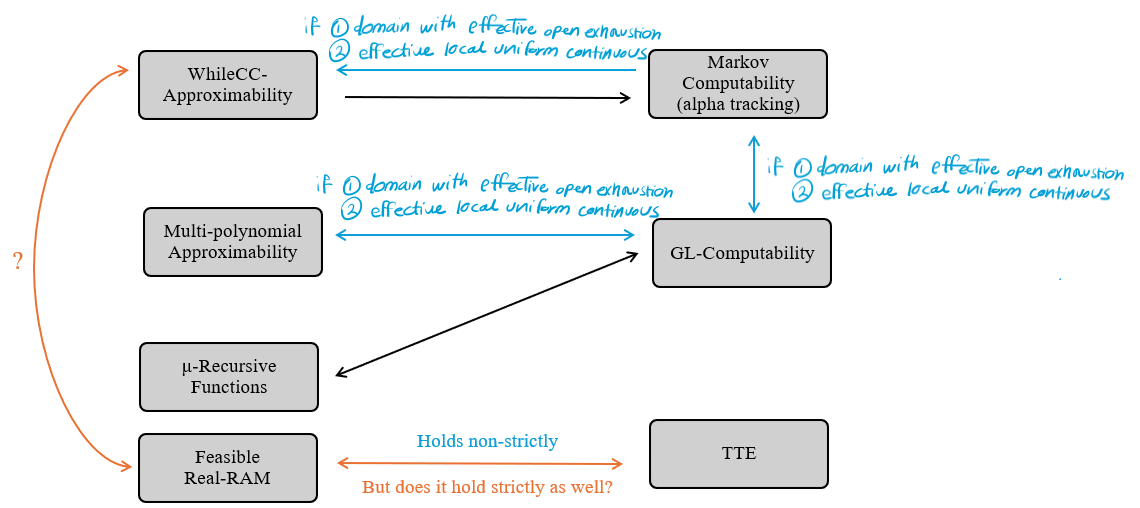
\includegraphics[width=.7\linewidth]{todo.png}
    % \end{center}
\end{frame}